\documentclass[12pt, twoside]{article}
\usepackage[letterpaper, margin=1in, headsep=0.5in]{geometry}
\usepackage[english]{babel}
\usepackage[utf8]{inputenc}
\usepackage{amsmath}
\usepackage{amsfonts}
\usepackage{amssymb}
\usepackage{tikz}
\usepackage{yhmath}
\usetikzlibrary{quotes, angles}
\usepackage{graphicx}
\usepackage{enumitem}
\usepackage{multicol}

\newif\ifmeta
\metatrue %print standards and topics tags

\title{Regents Geometry}
\author{Chris Huson}
\date{May 2022}

\usepackage{fancyhdr}
\pagestyle{fancy}
\fancyhf{}
\renewcommand{\headrulewidth}{0pt} % disable the underline of the header
\raggedbottom

\fancyhead[LE]{\thepage}
\fancyhead[RO]{\thepage \\ Name: \hspace{4cm} \,\\}
\fancyhead[LO]{BECA / Dr. Huson / Geometry\\* Unit 11: Function transformations\\* 16 May 2022}

\begin{document}
\subsubsection*{11.13 Exit Quiz: Function identification \hfill HSF.BF.B.3}
Identify each function with its name and the equation of its parent (simplest example). \\(e.g. line, parabola, square root, absolute value, reciprocal, circle, sine)
\begin{enumerate}
\item 
\begin{multicols}{2}
  Name: \\[1.5cm]
  Equation: 
  \columnbreak
  \begin{center}
    \begin{tikzpicture}
      \draw [thick, <->] (-3.4,0) -- (3.4,0) node [right] {$x$};
      \draw [thick, ->] (0,-0.5)--(0,3.4) node [left] {$y$};  
      \draw [thick,<->,samples=90,domain=-2.5:2.5] plot(\x,abs{\x});
    \end{tikzpicture}
  \end{center}
\end{multicols}

\item 
\begin{multicols}{2}
  Name: \\[2cm]
  Equation: 
  \columnbreak
  \begin{center}
    \begin{tikzpicture}
      \draw [thick, <->] (-3.4,0) -- (3.4,0) node [right] {$x$};
      \draw [thick, ->] (0,-2.5)--(0,2.4) node [left] {$y$};  
      \draw [thick,<->,samples=20,domain=-3.2:-0.5] plot(\x,1/\x);
      \draw [thick,<->,samples=20,domain=0.4:3.2] plot(\x,1/\x);
    \end{tikzpicture}
  \end{center}
\end{multicols}

\item 
\begin{multicols}{2}
  Name: \\[1.5cm]
  Equation: 
  \columnbreak
  \begin{center}
    \begin{tikzpicture}
      \draw [thick, <->] (-1.4,0) -- (5.4,0) node [right] {$x$};
      \draw [thick, ->] (0,-0.5)--(0,3.4) node [left] {$y$};  
      \draw [thick,->,samples=90,domain=0:5] plot(\x,{(\x)^0.5});
    \end{tikzpicture}
  \end{center}
\end{multicols}

\item 
\begin{multicols}{2}
  Name: \\[2cm]
  Equation: 
  \columnbreak
  \begin{center}
    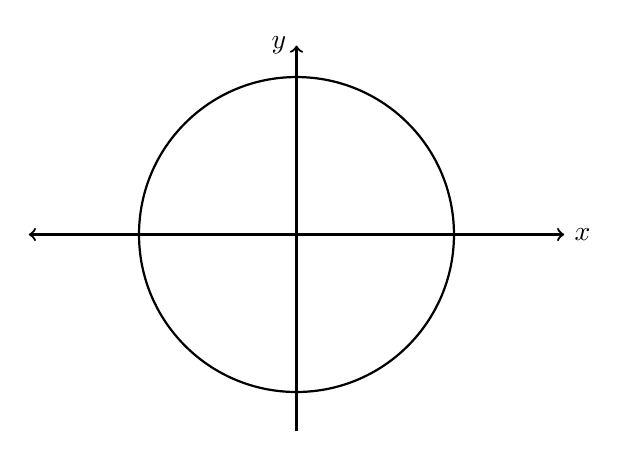
\begin{tikzpicture}
      \draw [thick, <->] (-3.4,0) -- (3.4,0) node [right] {$x$};
      \draw [thick, ->] (0,-2.5)--(0,2.4) node [left] {$y$};  
      \draw [thick,<->] (0,0) circle[radius=2cm];
    \end{tikzpicture}
  \end{center}
\end{multicols}

\newpage
\item 
\begin{multicols}{2}
  Name: \\[1.2cm]
  Equation: 
  \columnbreak
  \begin{center}
    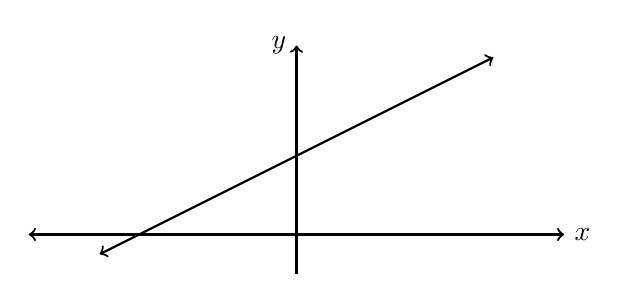
\begin{tikzpicture}
      \draw [thick, <->] (-3.4,0) -- (3.4,0) node [right] {$x$};
      \draw [thick, ->] (0,-0.5)--(0,2.4) node [left] {$y$};  
      \draw [thick,<->,samples=20,domain=-2.5:2.5] plot(\x,0.5*\x+1);
    \end{tikzpicture}
  \end{center}
\end{multicols}

\item 
\begin{multicols}{2}
  Name: \\[2cm]
  Equation: 
  \columnbreak
  \begin{center}
    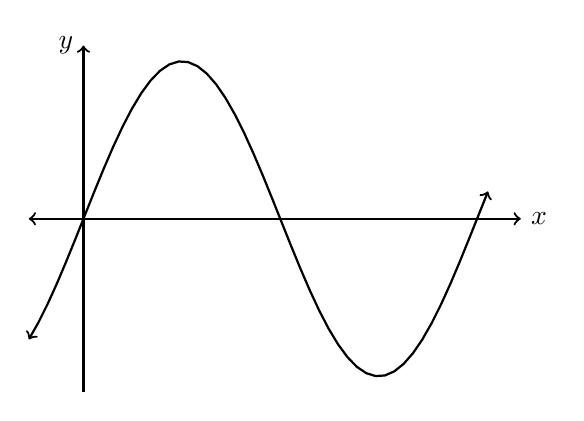
\begin{tikzpicture}[xscale=5/360, yscale=2]
      \draw [thick, <->] (-50,0) -- (400,0) node [right] {$x$};
      \draw [thick, ->] (0,-1.1)--(0,1.1) node [left] {$y$};  
      \draw [thick,<->,samples=50,domain=-50:370] plot(\x,{sin(\x)});
    \end{tikzpicture}
  \end{center}
\end{multicols}

\item 
\begin{multicols}{2}
  Name: \\[1.5cm]
  Equation: 
  \columnbreak
  \begin{center}
    \begin{tikzpicture}
      \draw [thick, <->] (-3.4,0) -- (3.4,0) node [right] {$x$};
      \draw [thick, ->] (0,-0.5)--(0,3.4) node [left] {$y$};  
      \draw [thick,<->,samples=20,domain=-1.8:1.8] plot(\x,{(\x-0)^2});
    \end{tikzpicture}
  \end{center}
\end{multicols}

\begin{multicols}{2}
  \item Graph the equation $y+1=(x-2)^2$ on the grid at right for $-1 \le x \le 5$.
  \begin{enumerate}
    \item Mark and label the vertex as a coordinate pair.
    \item Write down the $x$-intercepts.\vspace{1cm}
    \item Mark and label the $y$-intercept. 
    \item Draw the axis of symmetry and label it with its equation. \vspace{2cm}
  \end{enumerate}
  \begin{flushright} 
    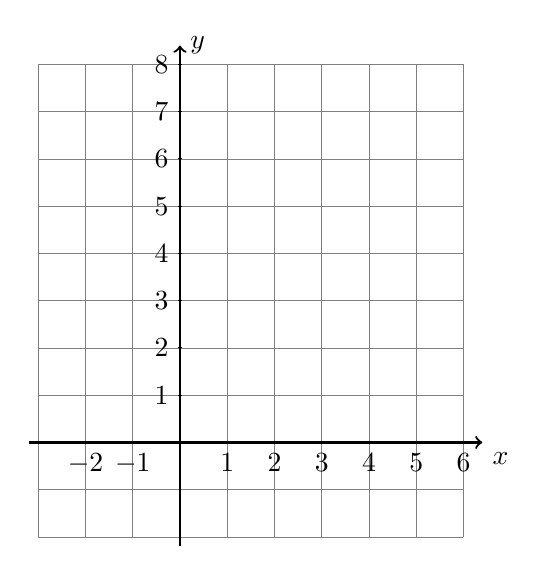
\begin{tikzpicture}[scale=0.6]
      \draw [help lines] (-3,-2) grid (6,8);
      \draw [thick, ->] (-3.2,0) -- (6.4,0) node [below right] {$x$};
      \draw [thick, ->] (0,-2.2)--(0,8.4) node [right] {$y$};
      \foreach \x in {-2,-1,1,2,...,6} \draw (\x cm,1pt)--(\x cm,-1pt) node[below] {$\x$};
      \foreach \y in {1,...,8} \draw (1pt,\y cm)--(-1pt,\y cm) node[left] {$\y$};
      %\fill (1,1) circle[radius=0.1];
    \end{tikzpicture}
    \end{flushright}
\end{multicols}



\end{enumerate}
\end{document}
  